\section{Scenario 4}
Daniele is keen for soccer, he loves to watch his team on tv. He wants to check on TIM website if they have any offer about tv services.

\begin{enumerate}
	\item He goes on \url{www.tim.it}
	\item He clicks on "TIM Premium Online" \url{www.tim.it/smart-life/tv-entertainment/tv/timpremiumonline}
	\item He scrolls through the site. He is interested in Serie A so he clicks on "Serie A TIM" in the top right part \url{www.tim.it/smart-life/tv-entertainment/serie-a}
	\item He clicks on "Serie A TIM TV" \url{www.tim.it/smart-life/tv-entertainment/serie-tim-tv}
	\item Daniele reads through the page but he doesn't like the offer. He clicks on "TIM" logo then "TIM Premium Online"
	\item He clicks on "ATTIVA CON OPERATORE" and enters his phone number. The services will be activated telephonically
\end{enumerate}

\newpage

\subsection{Results}
\begin{enumerate}
	
%------------------------------------------------------------------------------------------------------
	
\item Report on \url{www.tim.it/smart-life/tv-entertainment/tv/timpremiumonline}

\begin{center}
	
\includegraphics[width=\textwidth]{Screenshot/premium.jpg}
\end{center}
\vspace{1cm}

	\paragraph*{Content heuristics \\ Text}
	\begin{itemize}
		\item accuracy: satisfied
		\item currency: \textcolor{red}{severely violated}\\
		the user cannot know if the page is updated
		\item coverage: satisfied
		\item content objectivity: satisfied
		\item authority: satisfied
		\item conciseness: satisfied		
	\end{itemize}
	
	\paragraph*{General communication quality}
	\begin{itemize}
		\item text errors: satisfied
		\item multimedia consistency: satisfied
	\end{itemize}

	\paragraph*{Navigation heuristics \\ Navigation within a topic}
	\begin{itemize}
		\item segmentation: satisfied\\
		the information of the topic are organized in sections on the same page
	\end{itemize}	
	
	\paragraph*{Navigation within a transition}
	\begin{itemize}
		\item transition list: n/a
	\end{itemize}
	
	\paragraph*{Navigation within a group of topics}
	\begin{itemize}
		\item introduction list: n/a
		\item group navigation: \textcolor{orange}{partially violated}\\
		the user can reach the items related to the group (in the top-right part) but he/she can't reach the group by the site structure path
	\end{itemize}
	
	\paragraph*{Backward navigation}
	\begin{itemize}
		\item go back: \textcolor {orange}{partially violated}\\
		there isn't a "go back" functionality but the user can exploit the TIM logo to return to the homepage
	\end{itemize}
	
	\paragraph*{Overall navigation}
	\begin{itemize}
		\item landmarks: satisfied\\
		they are well visible on the top-right corner of the website
		\item link consistency: satisfied
		\item orientation clues: satisfied\\
		under the logo there is a site structure path
		\item orientation clues - topic: \textcolor{red}{severely violated}\\
		the user doesn't know the section he/she is visiting
		\item group orientation clues:  \textcolor{red}{severely violated}\\
		the user cannot know which group of topics he/she is visiting ("TV \& Entertainment")
		\item transition orientation clues: n/a
	\end{itemize}	
	
	\paragraph*{Visual and semantic heuristics \\ Overall graphic design }
	\begin{itemize}
		\item visual identity: satisfied
		\item chromatic code consistency: satisfied
		\item background contrast: satisfied
		\item font size: satisfied
		\item font color: satisfied
		\item font type: satisfied
		\item anchor identity: satisfied
		\item anchor states: satisfied
		\item icon consistency: satisfied
	\end{itemize}
	
	\paragraph*{Page layout}
	\begin{itemize}
		\item visual proximity: satisfied
		\item layout conventions: satisfied
		\item semiotics: satisfied
	\end{itemize}	
	
	\paragraph*{Cognitive heuristics \\ Single page}
	\begin{itemize}
		\item information overload: \textcolor{orange}{partially violated}\\
		this page is rich of content due to the importance of the topic (a user would like to know everything about a promotion)
	\end{itemize}	
	
	\paragraph*{Information architecture}
	\begin{itemize}
		\item classification adequacy within group of topics: n/a
		\item website mental map: satisfied
	\end{itemize}

\newpage

%------------------------------------------------------------------------------------------------------

\item Report on \url{www.tim.it/smart-life/tv-entertainment/serie-a}

\begin{center}
	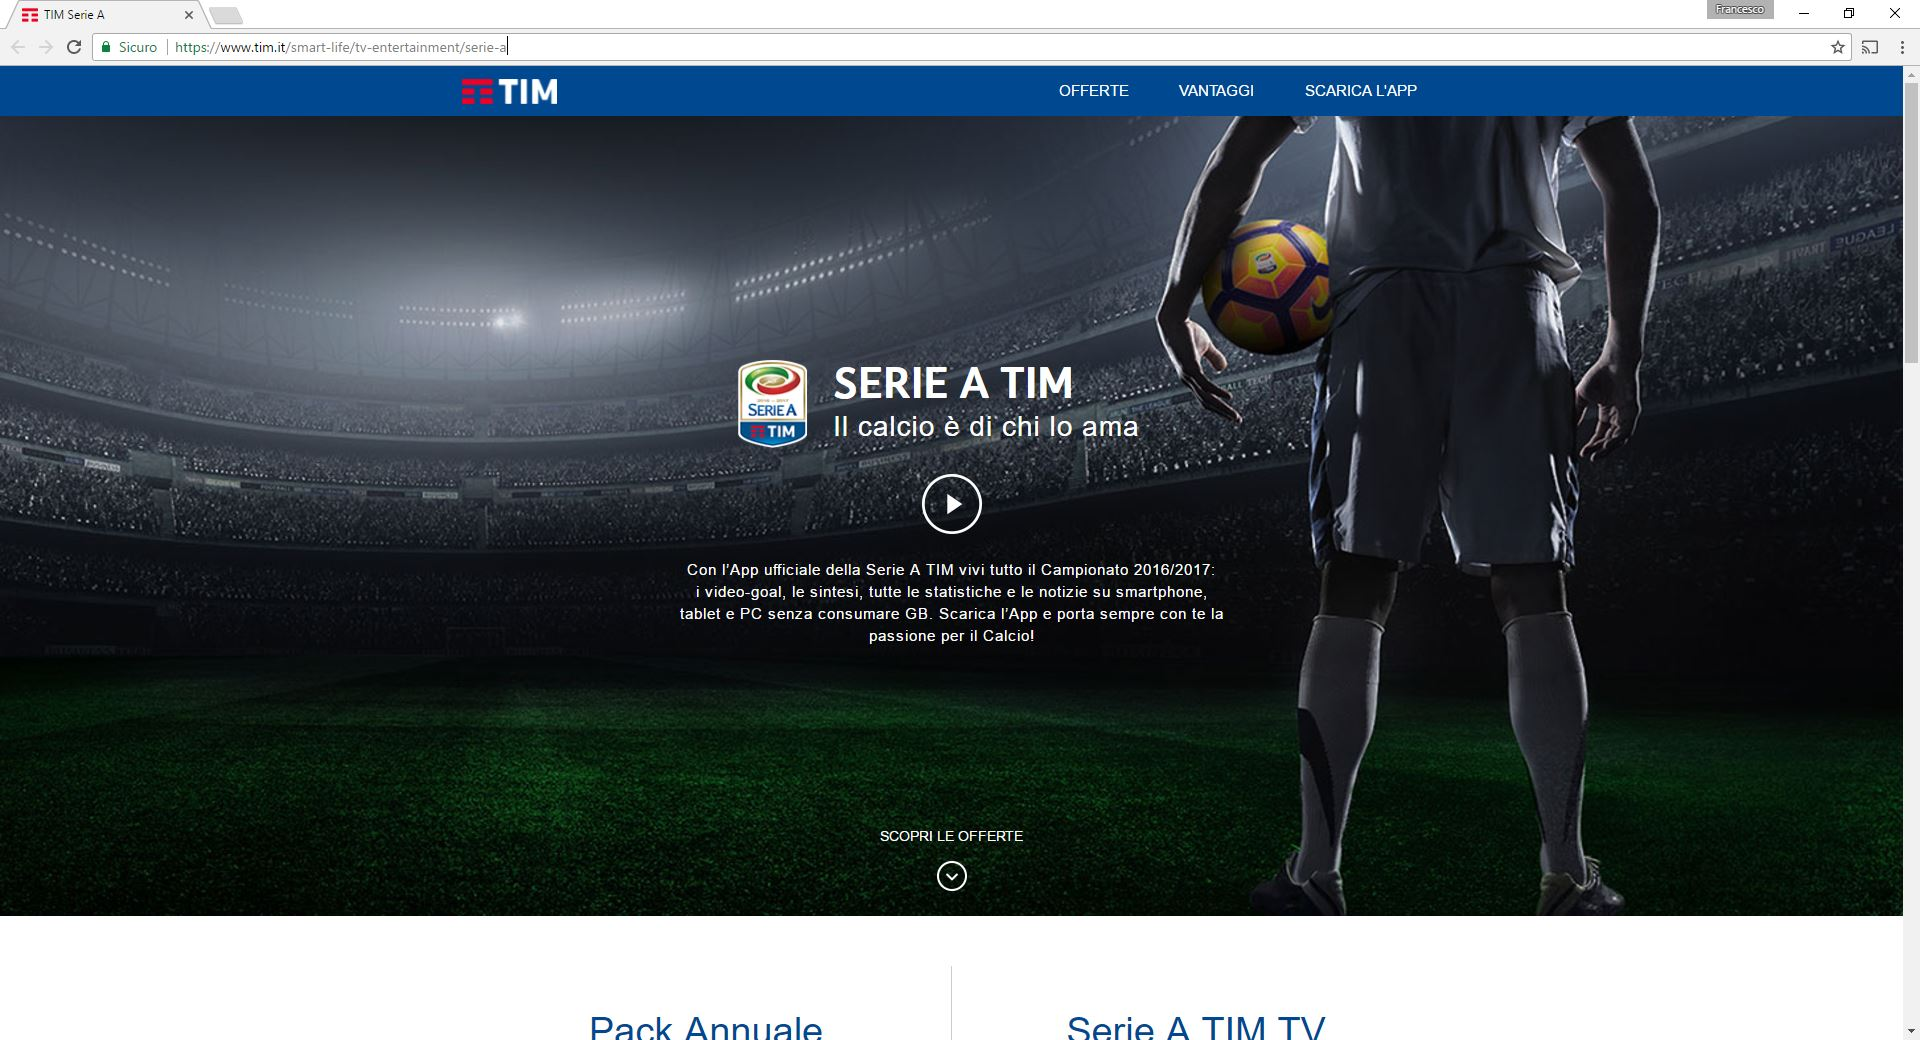
\includegraphics[width=\textwidth]{Screenshot/seriea.jpg}
\end{center}
\vspace{1cm}

	\paragraph*{Content heuristics \\ Text}
	\begin{itemize}
		\item accuracy: satisfied
		\item currency:  \textcolor{red}{severely violated}\\
		the user cannot know if the page is updated
		\item coverage: satisfied
		\item content objectivity: satisfied
		\item authority: satisfied
		\item conciseness: satisfied		
	\end{itemize}

	\paragraph*{General communication quality}
	\begin{itemize}
		\item text errors: satisfied
		\item multimedia consistency: satisfied
	\end{itemize}

	\paragraph*{Navigation heuristics \\ Navigation within a topic}
	\begin{itemize}
		\item segmentation: satisfied\\
		the information of the topic are organized in sections on the same page
	\end{itemize}	
	
	\paragraph*{Navigation within a transition}
	\begin{itemize}
		\item transition list: n/a
	\end{itemize}
	
	\paragraph*{Navigation within a group of topics}
	\begin{itemize}
		\item introduction list: n/a
		\item group navigation: \textcolor{orange}{partially violated}\\
		the user can reach the items related to the group ("SCOPRI LE OFFERTE") but he/she can't reach the group by the site structure path 
	\end{itemize}

	\paragraph*{Backward navigation}
	\begin{itemize}
		\item go back: \textcolor {red}{severely violated}\\
		there isn't a "go back" functionality and the user can only exploit the TIM logo to return to the homepage and redo the step
	\end{itemize}
	
	\paragraph*{Overall navigation}
	\begin{itemize}
		\item landmarks: \textcolor {red}{severely violated}\\
		there are no landmarks
		\item link consistency: satisfied
		\item orientation clues: \textcolor {red}{severely violated}\\
		the user cannot know where he/she is, there are no path
		\item orientation clues - topic: \textcolor{red}{severely violated}\\
		the user doesn't know the section he/she is visiting
		\item group orientation clues: \textcolor{red}{severely violated}\\
		the user cannot know which group of topics he/she is visiting ("TV \& Entertainment")
		\item transition orientation clues: n/a
	\end{itemize}	
	
	\paragraph*{Visual and semantic heuristics \\ Overall graphic design }
	\begin{itemize}
		\item visual identity: satisfied
		\item chromatic code consistency: satisfied
		\item background contrast: satisfied
		\item font size: satisfied
		\item font color: satisfied
		\item font type: satisfied
		\item anchor identity: satisfied
		\item anchor states: satisfied
		\item icon consistency: satisfied
	\end{itemize}
	
	\paragraph*{Page layout}
	\begin{itemize}
		\item visual proximity: satisfied
		\item layout conventions: satisfied
		\item semiotics: satisfied
	\end{itemize}	
	
	\paragraph*{Cognitive heuristics \\ Single page}
	\begin{itemize}
		\item information overload: satisfied
	\end{itemize}	
	
	\paragraph*{Information architecture}
	\begin{itemize}
		\item classification adequacy within group of topics: n/a
		\item website mental map: satisfied
	\end{itemize}

\newpage

%------------------------------------------------------------------------------------------------------

\item Report on \url{www.tim.it/smart-life/tv-entertainment/serie-tim-tv}

\begin{center}
	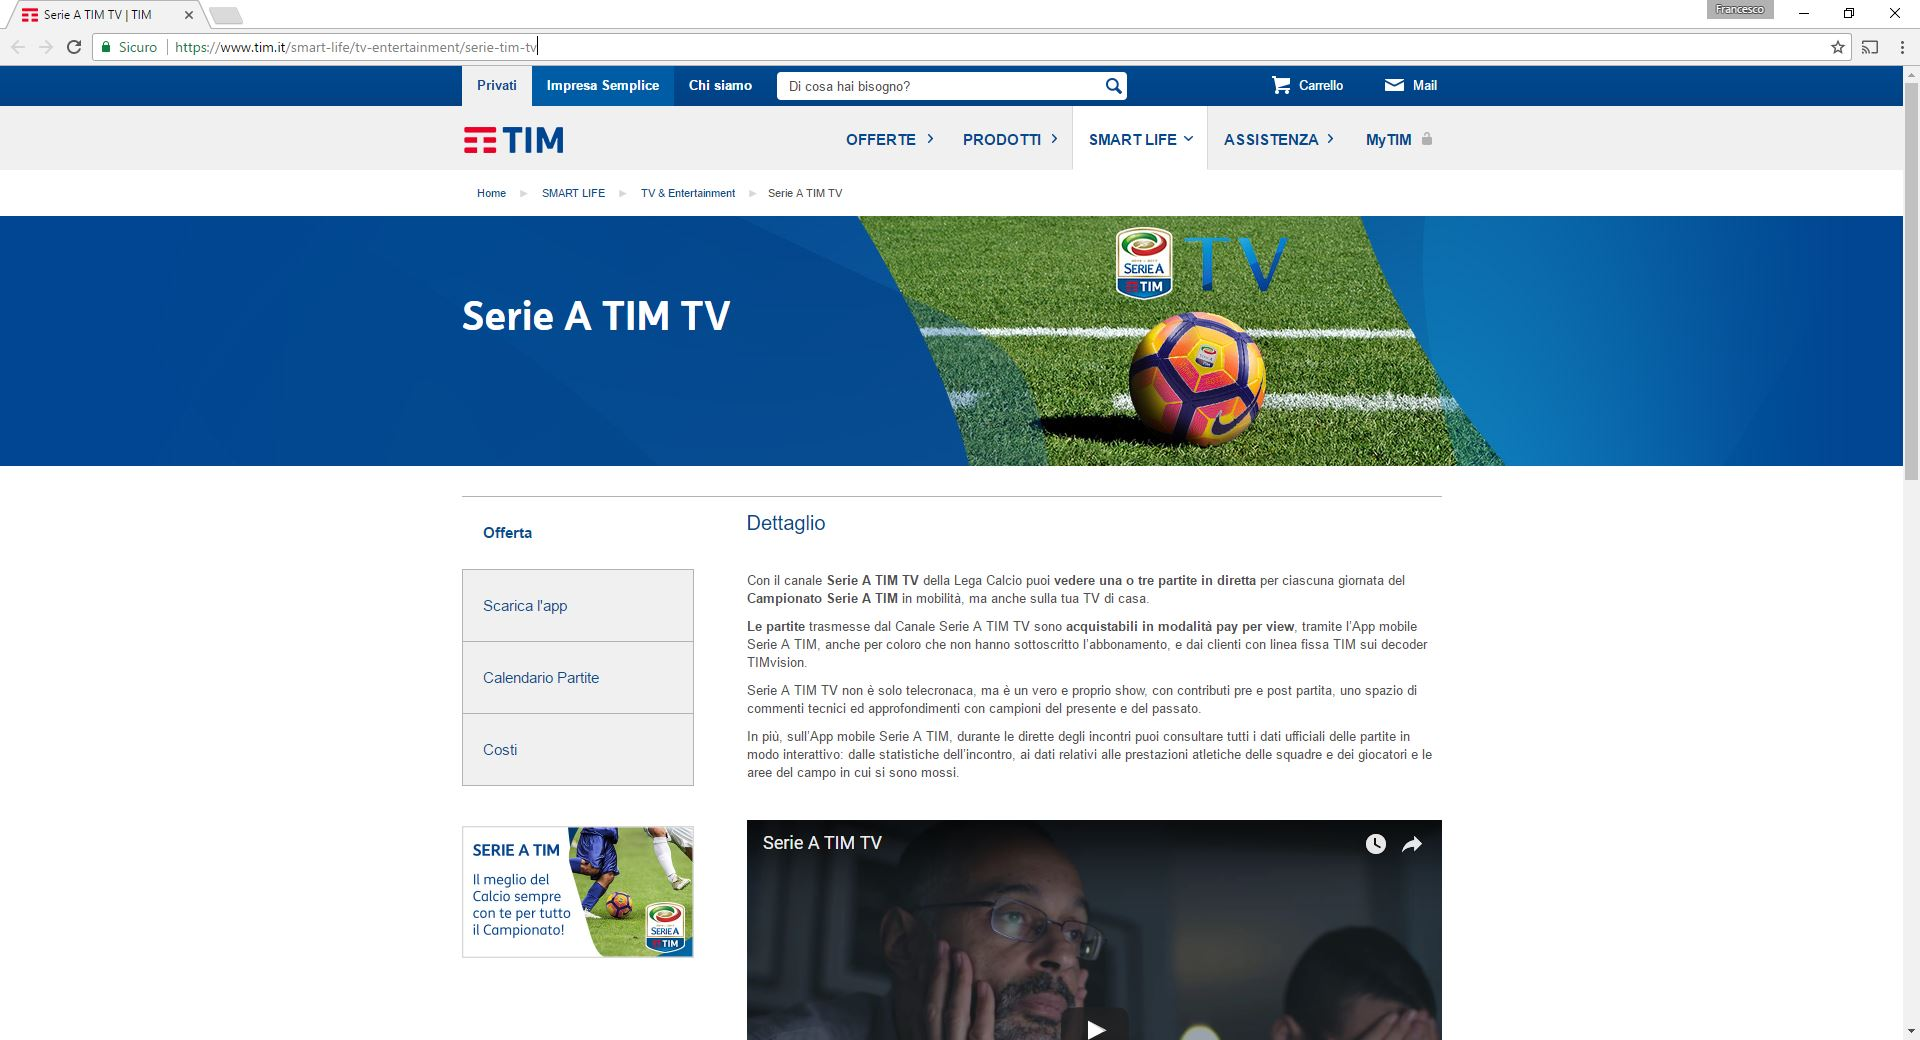
\includegraphics[width=\textwidth]{Screenshot/serieatimtv.jpg}
\end{center}
\vspace{1cm}

	\paragraph*{Content heuristics \\ Text}
	\begin{itemize}
		\item accuracy: satisfied
		\item currency: \textcolor{red}{severely violated}\\
		the user cannot know if the page is updated
		\item coverage: satisfied
		\item content objectivity: satisfied
		\item authority: satisfied
		\item conciseness: satisfied		
	\end{itemize}
	
	\paragraph*{General communication quality}
	\begin{itemize}
		\item text errors: satisfied
		\item multimedia consistency: satisfied
	\end{itemize}
	
	\paragraph*{Navigation heuristics \\ Navigation within a topic}
	\begin{itemize}
		\item segmentation: satisfied\\
		the information of the topic are organized in sub-sections on the same page 
	\end{itemize}	
	
	\paragraph*{Navigation within a transition}
	\begin{itemize}
		\item transition list: n/a
	\end{itemize}
	
	\paragraph*{Navigation within a group of topics}
	\begin{itemize}
		\item introduction list: n/a
		\item group navigation: \textcolor{orange}{partially violated}\\
		the user can reach the group by the site structure path but he/she can't reach items related to the group
	\end{itemize}
	
	\paragraph*{Backward navigation}
	\begin{itemize}
		\item go back: \textcolor{red}{severely violated}\\
		there is no "go back" functionality, the user can go to the homepage through the TIM logo or repeat the steps
	\end{itemize}
	
	\paragraph*{Overall navigation}
	\begin{itemize}
		\item landmarks: satisfied\\
		they are well visible on the top-right corner of the website 
		\item link consistency: satisfied
		\item orientation clues: \textcolor{orange}{partially violated}\\
		the user has a path structure that doesn't resemble his actions
		\item orientation clues - topic: satisfied\\
		the user knows the subsection he/she is visiting. When the user navigate through the site, the section's labels are well visible on the left of the page
		\item group orientation clues: satisfied
		\item transition orientation clues: n/a
	\end{itemize}	
	
	\paragraph*{Visual and semantic heuristics \\ Overall graphic design }
	\begin{itemize}
		\item visual identity: satisfied
		\item chromatic code consistency: satisfied
		\item background contrast: satisfied
		\item font size: satisfied
		\item font color: satisfied
		\item font type: satisfied
		\item anchor identity: satisfied
		\item anchor states: satisfied
		\item icon consistency: satisfied
	\end{itemize}
	
	\paragraph*{Page layout}
	\begin{itemize}
		\item visual proximity: satisfied
		\item layout conventions: satisfied
		\item semiotics: satisfied
	\end{itemize}	
	
	\paragraph*{Cognitive heuristics \\ Single page}
	\begin{itemize}
		\item information overload: satisfied
	\end{itemize}	

	\paragraph*{Information architecture}
	\begin{itemize}
		\item classification adequacy within group of topics: n/a
		\item website mental map: satisfied
	\end{itemize}
\end{enumerate}